\documentclass{article}
\usepackage{tikz}
\usetikzlibrary{arrows.meta}

\begin{document}

\begin{figure}[h]
    \centering
    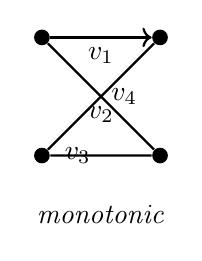
\begin{tikzpicture}[scale=1.5]
        % Nodes
        \node (v1) at (0, 0) [circle, fill, inner sep=2pt] {};
        \node (v2) at (1, 0) [circle, fill, inner sep=2pt] {};
        \node (v3) at (0, -1) [circle, fill, inner sep=2pt] {};
        \node (v4) at (1, -1) [circle, fill, inner sep=2pt] {};

        % Edges
        \draw[->, thick] (v1) -- node[below] {$v_1$} (v2);
        \draw[thick] (v2) -- node[below] {$v_2$} (v3);
        \draw[thick] (v3) -- node[left] {$v_3$} (v4);
        \draw[thick] (v4) -- node[right] {$v_4$} (v1);

        % Monotonic label
        \node at (0.5, -1.5) {\textit{monotonic}};
    \end{tikzpicture}
    \quad
    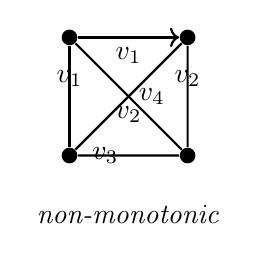
\begin{tikzpicture}[scale=1.5]
        % Nodes
        \node (v1) at (0, 0) [circle, fill, inner sep=2pt] {};
        \node (v2) at (1, 0) [circle, fill, inner sep=2pt] {};
        \node (v3) at (0, -1) [circle, fill, inner sep=2pt] {};
        \node (v4) at (1, -1) [circle, fill, inner sep=2pt] {};

        % Edges
        \draw[->, thick] (v1) -- node[below] {$v_1$} (v2);
        \draw[thick] (v2) -- node[below] {$v_2$} (v3);
        \draw[thick] (v3) -- node[left] {$v_3$} (v4);
        \draw[thick] (v4) -- node[right] {$v_4$} (v1);
        \draw[thick] (v1) -- node[above] {$v_1$} (v3);
        \draw[thick] (v2) -- node[above] {$v_2$} (v4);

        % Non-monotonic label
        \node at (0.5, -1.5) {\textit{non-monotonic}};
    \end{tikzpicture}
\end{figure}

\end{document}